
\documentclass[a4paper,11pt]{article}
\usepackage{geometry}
\geometry{margin=2cm}
\usepackage{booktabs}
\usepackage{graphicx}
\usepackage{amsmath}
\usepackage{siunitx}
\usepackage{caption}
\usepackage{times}
\usepackage[utf8]{inputenc}
\usepackage{tocloft}
\usepackage{rotating} % Untuk mendukung landscape

\title{Spectral Simulation Report}
\author{Automated Analysis}
\date{\today}

\begin{document}

\maketitle
\tableofcontents
\clearpage

\section{Introduction}
This report presents the results of spectral simulations derived from HDF5 dataset analysis. Each sample includes a spectral plot displayed in a full horizontal page and a detailed table summarizing the initial composition, actual positions, total pixels, and signal-to-noise ratio (SNR), along with simulation parameters such as temperature and electron density.


\section{Sample: 11469}
\subsection{Simulation Parameters}
\begin{table}[h!]
    \centering
    \begin{tabular}{ll}
        \toprule
        \textbf{Parameter} & \textbf{Value} \\
        \midrule
        Temperature ($T$) & 8838 \,\si{K} \\
        Electron Density ($n_e$) & 2.78e+14 \,\si{cm^-3} \\
        Total Pixels & 4096 \\
        Signal-to-Noise Ratio (SNR) & 33.36 \\
        \bottomrule
    \end{tabular}
    \caption{Simulation parameters and additional metrics for sample 11469.}
    \label{tab:params_11469}
\end{table}

\subsection{Composition Analysis}
\begin{table}[h!]
    \centering
    \begin{tabular}{lcc}
        \toprule
        \textbf{Element} & \textbf{Initial Composition (\%)} & \textbf{Actual Positions} \\
        \midrule
        Al & 2.61 & 399.0 \\
        Ar & 0.00 & 0.0 \\
        C & 0.00 & 0.0 \\
        Ca & 2.65 & 150.0 \\
        Cl & 7.36 & 35.0 \\
        Co & 5.62 & 1404.0 \\
        Cr & 5.09 & 397.0 \\
        Fe & 8.39 & 2738.0 \\
        Mg & 11.92 & 343.0 \\
        Mn & 10.31 & 706.0 \\
        N & 11.43 & 401.0 \\
        Na & 6.99 & 322.0 \\
        Ni & 9.78 & 478.0 \\
        O & 7.01 & 152.0 \\
        S & 4.43 & 207.0 \\
        Si & 3.73 & 220.0 \\
        Ti & 2.66 & 1183.0 \\
        background & N/A & 536.0 \\

        \midrule
        \textbf{Total Positions} & & 9671.0 \\
        \bottomrule
    \end{tabular}
    \caption{Composition analysis for sample 11469.}
    \label{tab:comp_11469}
\end{table}

\subsection{Spectral Plot}
\begin{figure}[p]
    \begin{landscape}
        \centering
        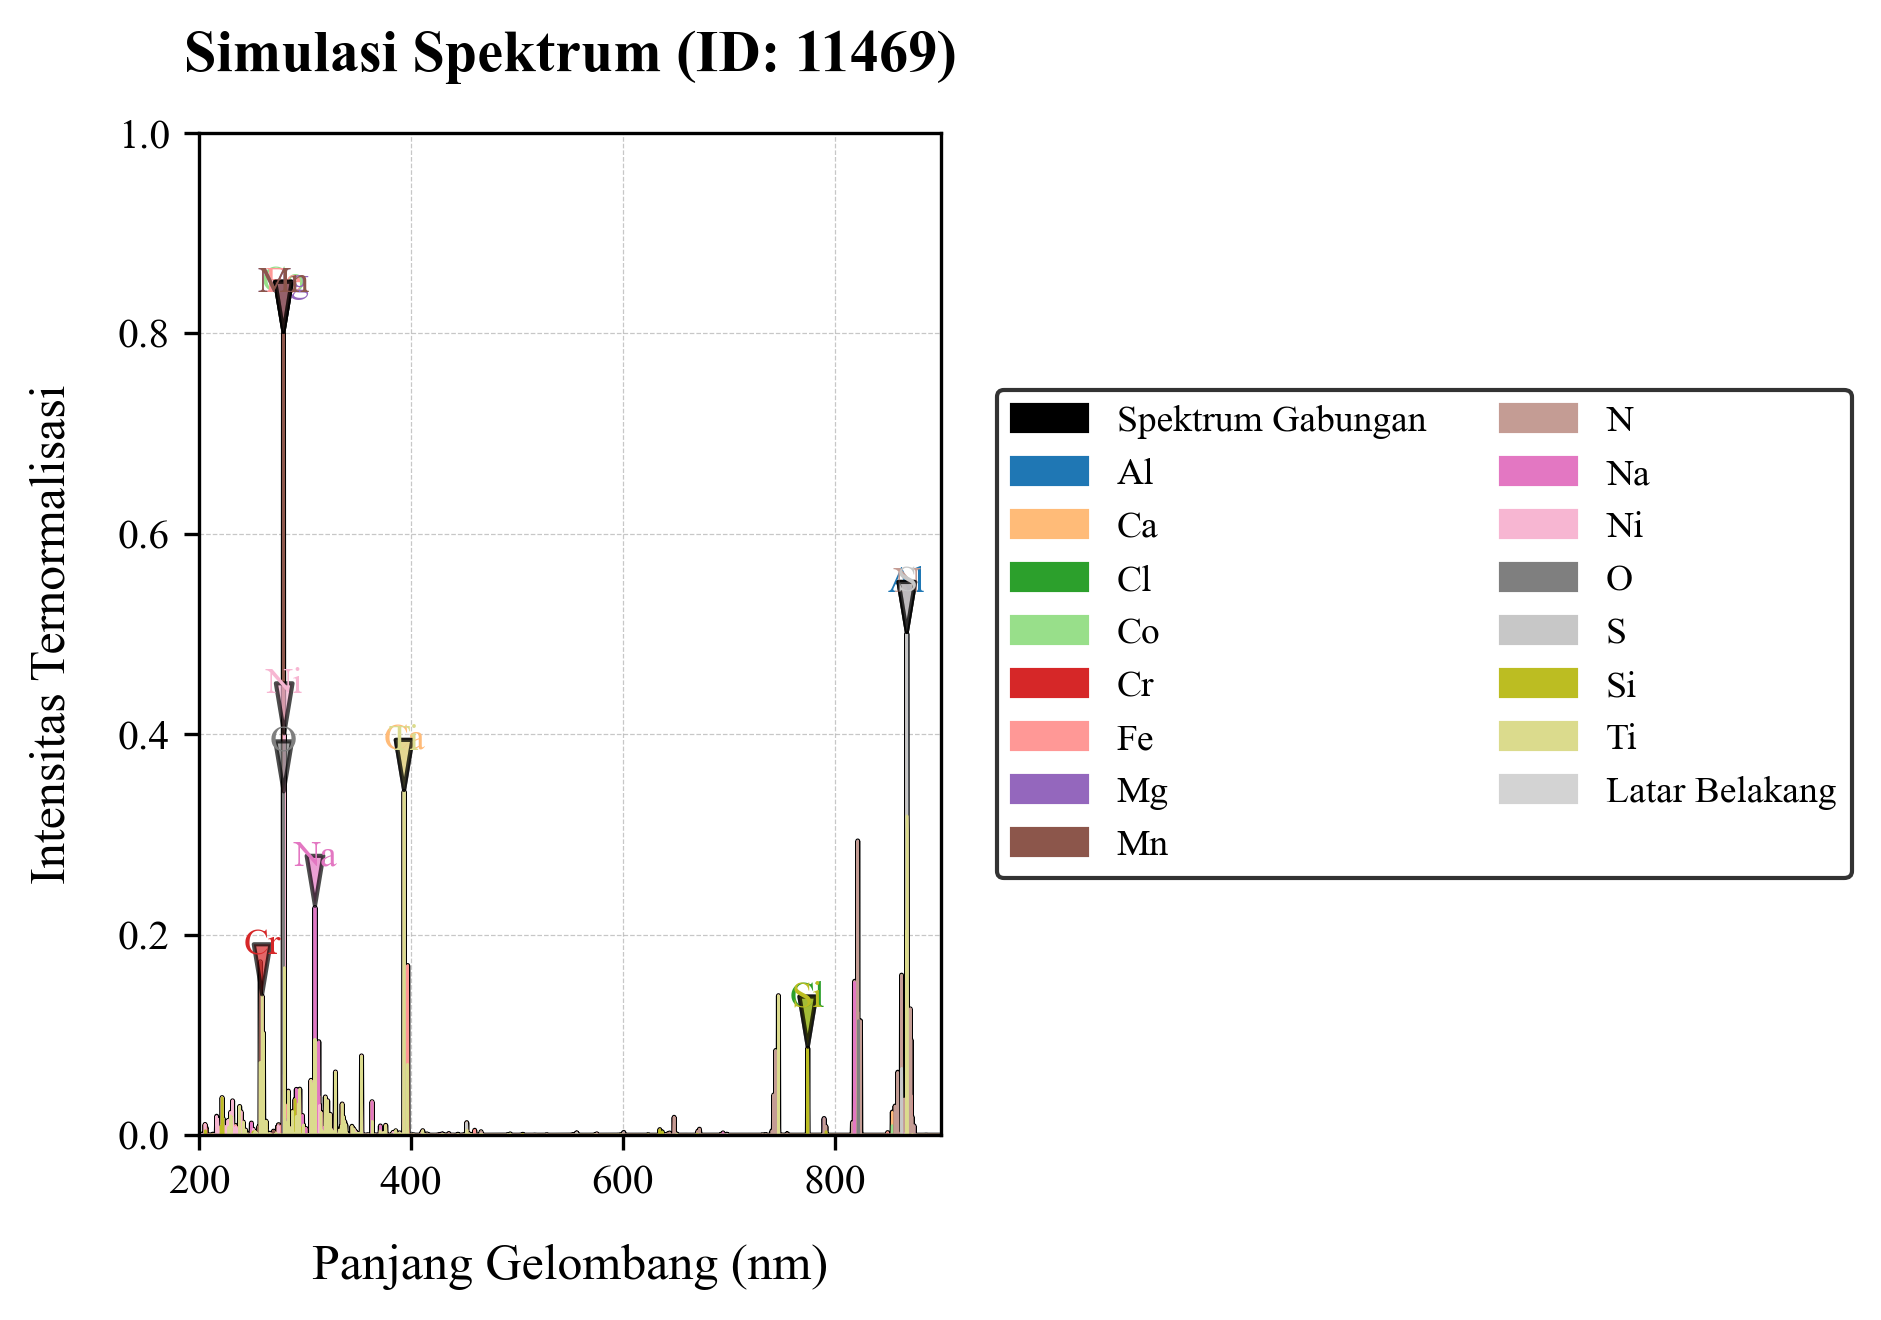
\includegraphics[width=\textwidth]{spectrum_11469.png}
        \caption{Spectral simulation plot for sample 11469 in full horizontal layout.}
        \label{fig:spectrum_11469}
    \end{landscape}
\end{figure}

\clearpage

\section{Sample: 9375}
\subsection{Simulation Parameters}
\begin{table}[h!]
    \centering
    \begin{tabular}{ll}
        \toprule
        \textbf{Parameter} & \textbf{Value} \\
        \midrule
        Temperature ($T$) & 10657 \,\si{K} \\
        Electron Density ($n_e$) & 1.38e+16 \,\si{cm^-3} \\
        Total Pixels & 4096 \\
        Signal-to-Noise Ratio (SNR) & 37.77 \\
        \bottomrule
    \end{tabular}
    \caption{Simulation parameters and additional metrics for sample 9375.}
    \label{tab:params_9375}
\end{table}

\subsection{Composition Analysis}
\begin{table}[h!]
    \centering
    \begin{tabular}{lcc}
        \toprule
        \textbf{Element} & \textbf{Initial Composition (\%)} & \textbf{Actual Positions} \\
        \midrule
        Al & 0.00 & 0.0 \\
        Ar & 0.00 & 0.0 \\
        C & 11.20 & 330.0 \\
        Ca & 14.63 & 150.0 \\
        Cl & 1.84 & 31.0 \\
        Co & 7.18 & 1404.0 \\
        Cr & 2.10 & 397.0 \\
        Fe & 11.57 & 2762.0 \\
        Mg & 14.76 & 356.0 \\
        Mn & 4.25 & 706.0 \\
        N & 0.00 & 0.0 \\
        Na & 3.38 & 322.0 \\
        Ni & 14.01 & 478.0 \\
        O & 0.00 & 0.0 \\
        S & 4.69 & 228.0 \\
        Si & 10.38 & 223.0 \\
        Ti & 0.00 & 0.0 \\
        background & N/A & 657.0 \\

        \midrule
        \textbf{Total Positions} & & 8044.0 \\
        \bottomrule
    \end{tabular}
    \caption{Composition analysis for sample 9375.}
    \label{tab:comp_9375}
\end{table}

\subsection{Spectral Plot}
\begin{figure}[p]
    \begin{landscape}
        \centering
        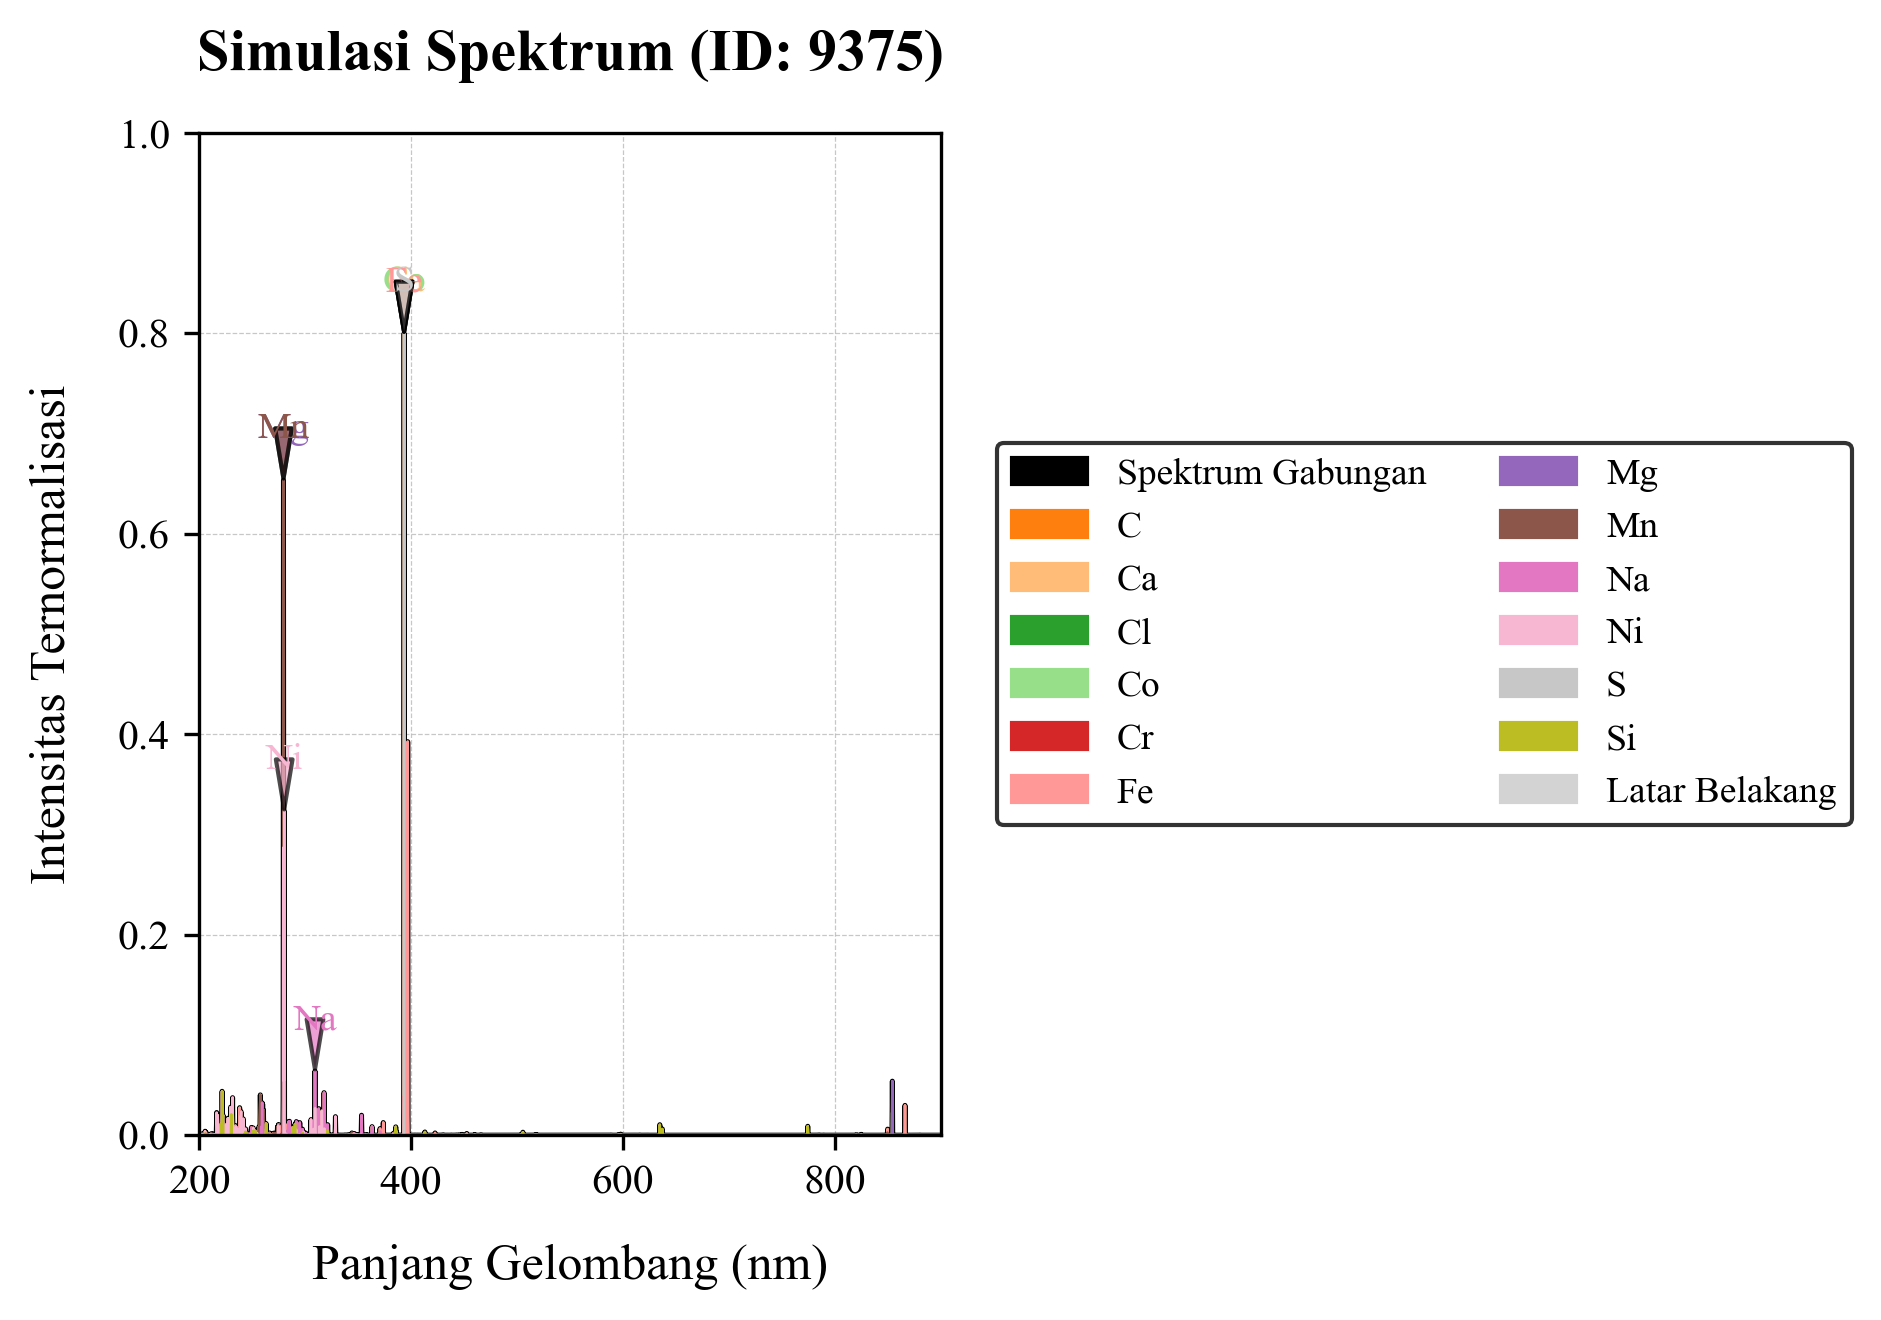
\includegraphics[width=\textwidth]{spectrum_9375.png}
        \caption{Spectral simulation plot for sample 9375 in full horizontal layout.}
        \label{fig:spectrum_9375}
    \end{landscape}
\end{figure}

\clearpage

\section{Sample: 5579}
\subsection{Simulation Parameters}
\begin{table}[h!]
    \centering
    \begin{tabular}{ll}
        \toprule
        \textbf{Parameter} & \textbf{Value} \\
        \midrule
        Temperature ($T$) & 6616 \,\si{K} \\
        Electron Density ($n_e$) & 1.56e+17 \,\si{cm^-3} \\
        Total Pixels & 4096 \\
        Signal-to-Noise Ratio (SNR) & 39.94 \\
        \bottomrule
    \end{tabular}
    \caption{Simulation parameters and additional metrics for sample 5579.}
    \label{tab:params_5579}
\end{table}

\subsection{Composition Analysis}
\begin{table}[h!]
    \centering
    \begin{tabular}{lcc}
        \toprule
        \textbf{Element} & \textbf{Initial Composition (\%)} & \textbf{Actual Positions} \\
        \midrule
        Al & 4.93 & 158.0 \\
        Ar & 6.15 & 286.0 \\
        C & 7.92 & 209.0 \\
        Ca & 10.45 & 150.0 \\
        Cl & 10.18 & 12.0 \\
        Co & 11.41 & 866.0 \\
        Cr & 8.33 & 397.0 \\
        Fe & 0.00 & 0.0 \\
        Mg & 2.98 & 161.0 \\
        Mn & 5.20 & 655.0 \\
        N & 4.46 & 396.0 \\
        Na & 11.70 & 330.0 \\
        Ni & 2.17 & 478.0 \\
        O & 7.67 & 50.0 \\
        S & 1.32 & 25.0 \\
        Si & 2.97 & 168.0 \\
        Ti & 2.14 & 1181.0 \\
        background & N/A & 1199.0 \\

        \midrule
        \textbf{Total Positions} & & 6721.0 \\
        \bottomrule
    \end{tabular}
    \caption{Composition analysis for sample 5579.}
    \label{tab:comp_5579}
\end{table}

\subsection{Spectral Plot}
\begin{figure}[p]
    \begin{landscape}
        \centering
        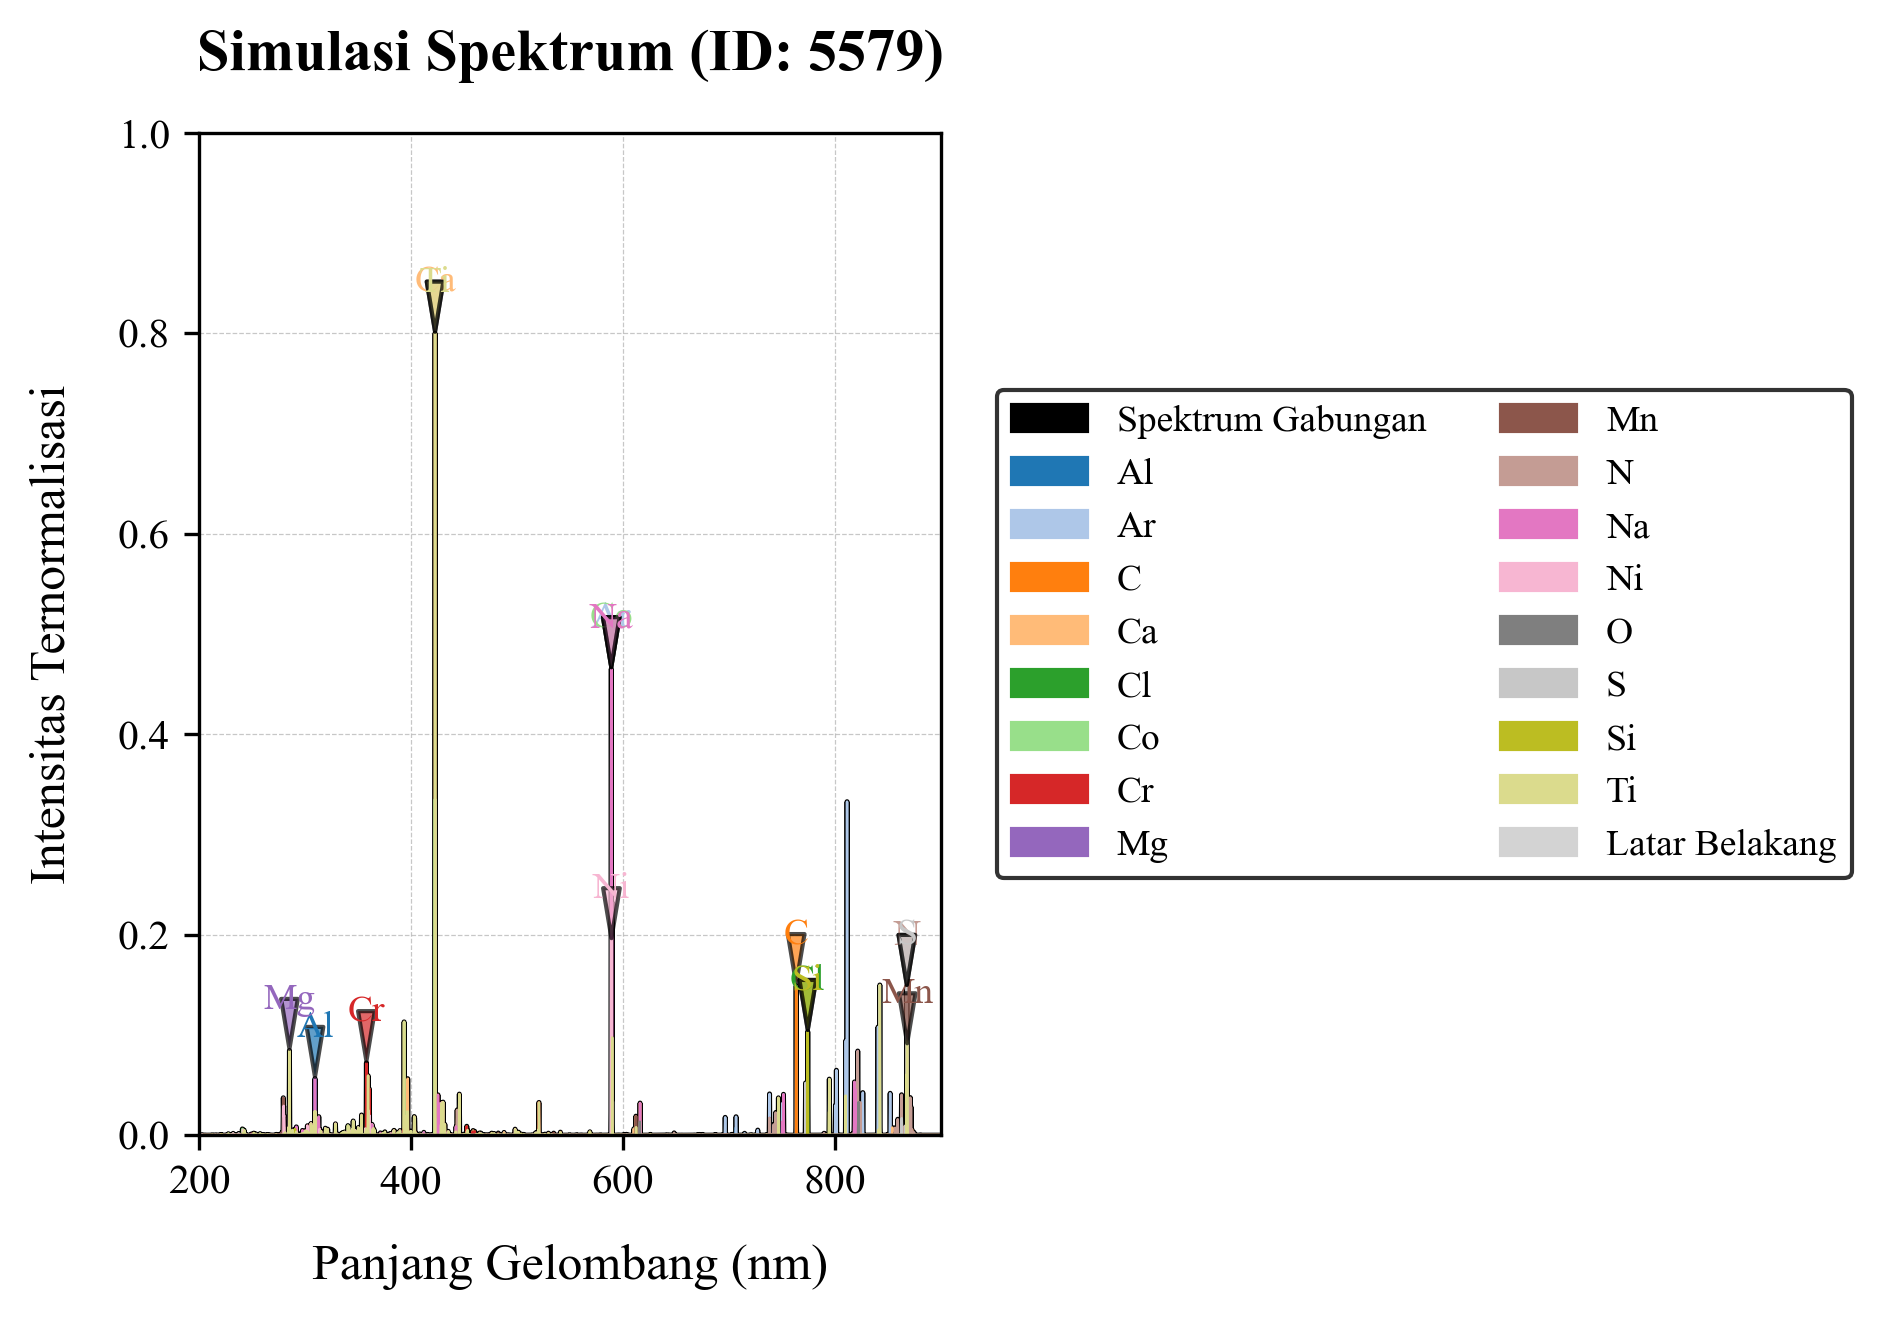
\includegraphics[width=\textwidth]{spectrum_5579.png}
        \caption{Spectral simulation plot for sample 5579 in full horizontal layout.}
        \label{fig:spectrum_5579}
    \end{landscape}
\end{figure}

\clearpage

\section{Sample: 17647}
\subsection{Simulation Parameters}
\begin{table}[h!]
    \centering
    \begin{tabular}{ll}
        \toprule
        \textbf{Parameter} & \textbf{Value} \\
        \midrule
        Temperature ($T$) & 6212 \,\si{K} \\
        Electron Density ($n_e$) & 1.48e+15 \,\si{cm^-3} \\
        Total Pixels & 4096 \\
        Signal-to-Noise Ratio (SNR) & 37.77 \\
        \bottomrule
    \end{tabular}
    \caption{Simulation parameters and additional metrics for sample 17647.}
    \label{tab:params_17647}
\end{table}

\subsection{Composition Analysis}
\begin{table}[h!]
    \centering
    \begin{tabular}{lcc}
        \toprule
        \textbf{Element} & \textbf{Initial Composition (\%)} & \textbf{Actual Positions} \\
        \midrule
        Al & 0.00 & 0.0 \\
        Ar & 12.05 & 408.0 \\
        C & 0.00 & 0.0 \\
        Ca & 10.73 & 150.0 \\
        Cl & 1.21 & 12.0 \\
        Co & 0.00 & 0.0 \\
        Cr & 16.37 & 397.0 \\
        Fe & 0.00 & 0.0 \\
        Mg & 10.56 & 184.0 \\
        Mn & 15.40 & 684.0 \\
        N & 0.00 & 0.0 \\
        Na & 4.13 & 322.0 \\
        Ni & 6.04 & 478.0 \\
        O & 0.00 & 0.0 \\
        S & 11.97 & 25.0 \\
        Si & 11.54 & 208.0 \\
        Ti & 0.00 & 0.0 \\
        background & N/A & 2102.0 \\

        \midrule
        \textbf{Total Positions} & & 4970.0 \\
        \bottomrule
    \end{tabular}
    \caption{Composition analysis for sample 17647.}
    \label{tab:comp_17647}
\end{table}

\subsection{Spectral Plot}
\begin{figure}[p]
    \begin{landscape}
        \centering
        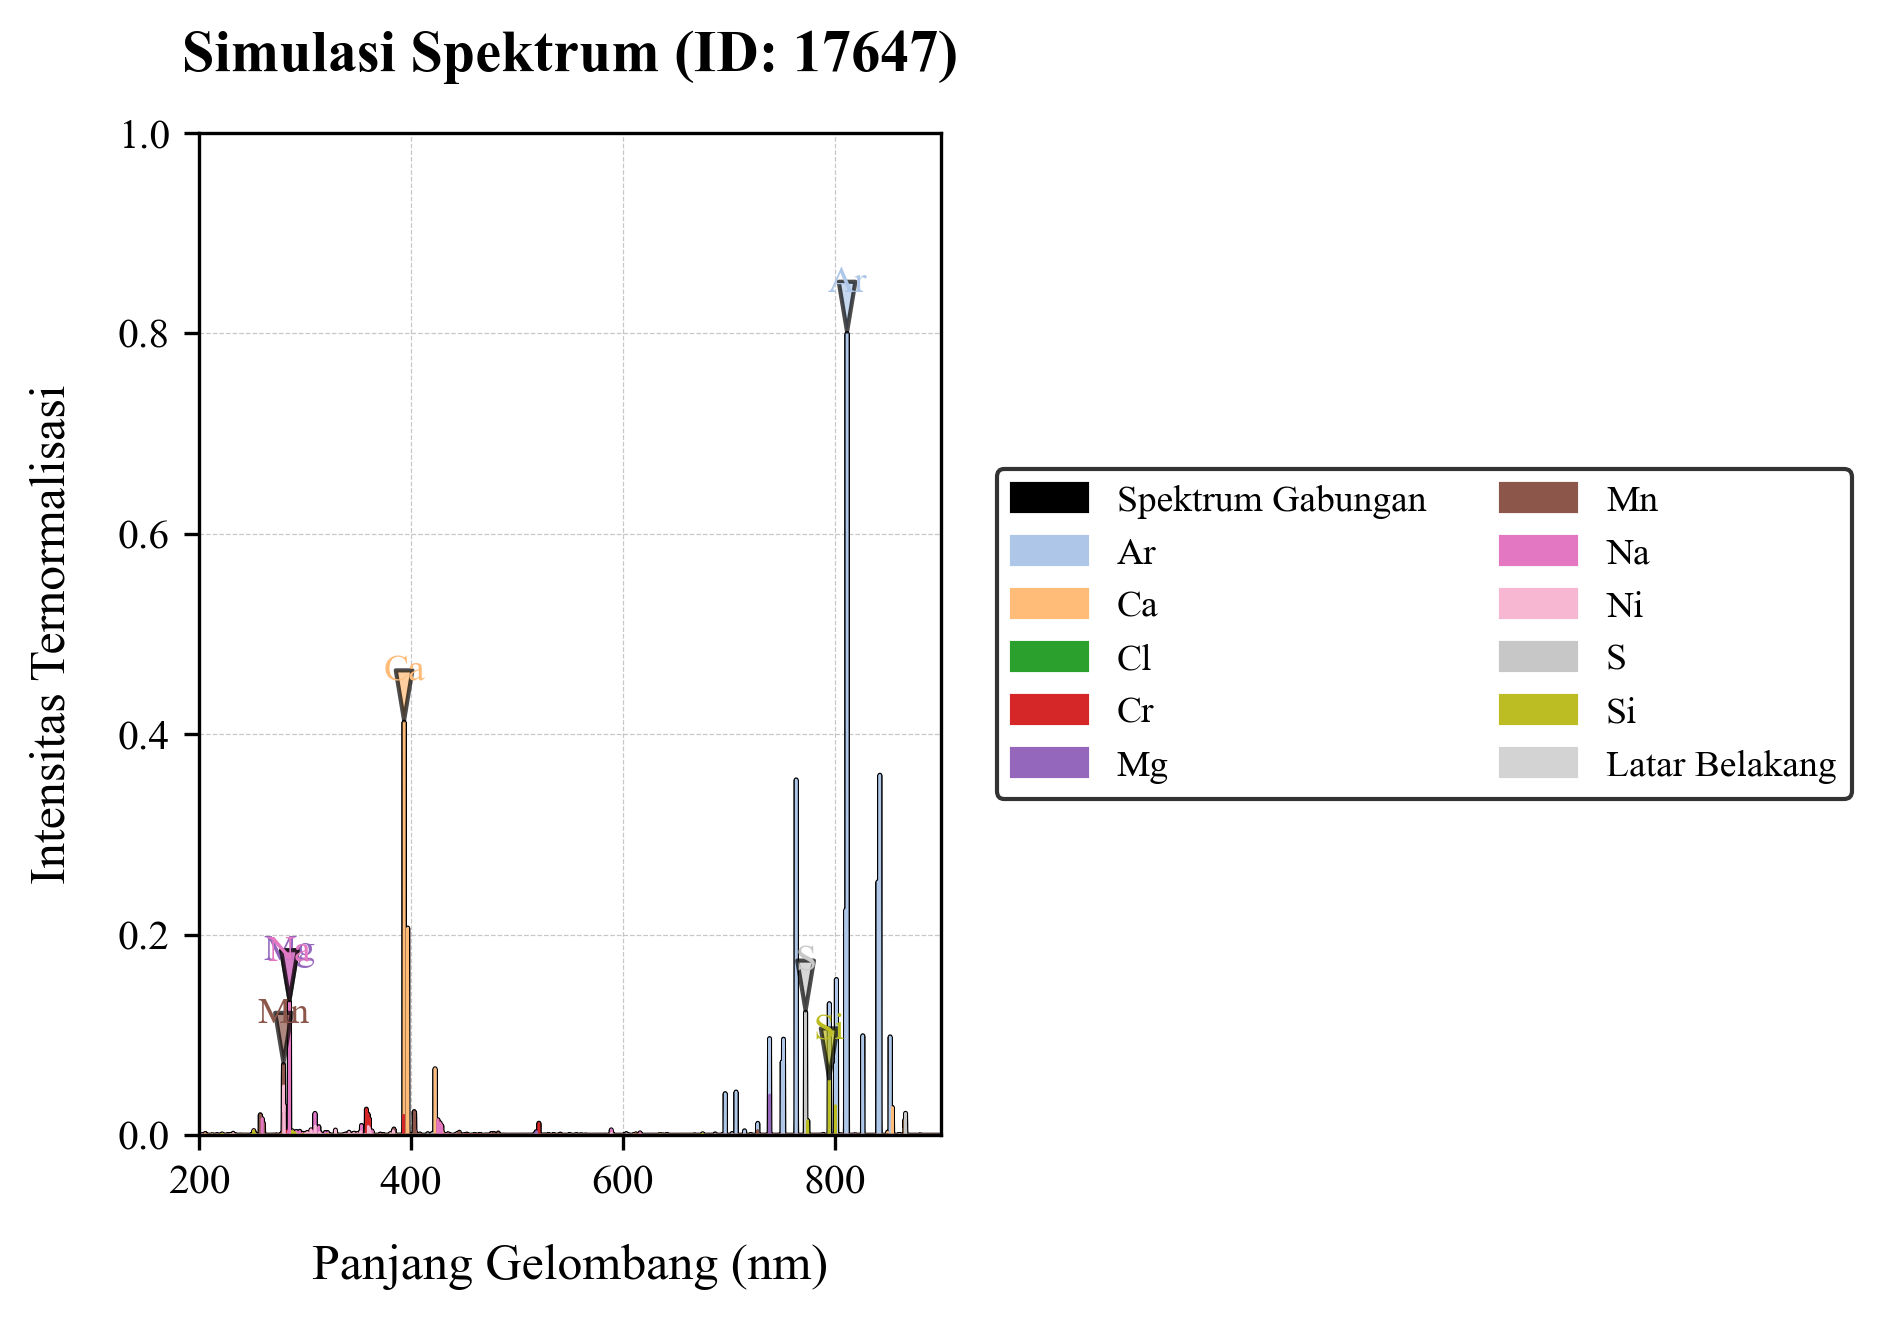
\includegraphics[width=\textwidth]{spectrum_17647.png}
        \caption{Spectral simulation plot for sample 17647 in full horizontal layout.}
        \label{fig:spectrum_17647}
    \end{landscape}
\end{figure}

\clearpage

\section{Sample: 17016}
\subsection{Simulation Parameters}
\begin{table}[h!]
    \centering
    \begin{tabular}{ll}
        \toprule
        \textbf{Parameter} & \textbf{Value} \\
        \midrule
        Temperature ($T$) & 5606 \,\si{K} \\
        Electron Density ($n_e$) & 4.23e+16 \,\si{cm^-3} \\
        Total Pixels & 4096 \\
        Signal-to-Noise Ratio (SNR) & 36.92 \\
        \bottomrule
    \end{tabular}
    \caption{Simulation parameters and additional metrics for sample 17016.}
    \label{tab:params_17016}
\end{table}

\subsection{Composition Analysis}
\begin{table}[h!]
    \centering
    \begin{tabular}{lcc}
        \toprule
        \textbf{Element} & \textbf{Initial Composition (\%)} & \textbf{Actual Positions} \\
        \midrule
        Al & 2.95 & 128.0 \\
        Ar & 9.73 & 246.0 \\
        C & 0.00 & 0.0 \\
        Ca & 11.22 & 150.0 \\
        Cl & 9.87 & 12.0 \\
        Co & 8.29 & 795.0 \\
        Cr & 12.37 & 397.0 \\
        Fe & 0.00 & 0.0 \\
        Mg & 0.68 & 135.0 \\
        Mn & 7.21 & 552.0 \\
        N & 0.00 & 0.0 \\
        Na & 7.37 & 330.0 \\
        Ni & 9.41 & 478.0 \\
        O & 5.47 & 8.0 \\
        S & 5.15 & 25.0 \\
        Si & 10.28 & 128.0 \\
        Ti & 0.00 & 0.0 \\
        background & N/A & 1995.0 \\

        \midrule
        \textbf{Total Positions} & & 5379.0 \\
        \bottomrule
    \end{tabular}
    \caption{Composition analysis for sample 17016.}
    \label{tab:comp_17016}
\end{table}

\subsection{Spectral Plot}
\begin{figure}[p]
    \begin{landscape}
        \centering
        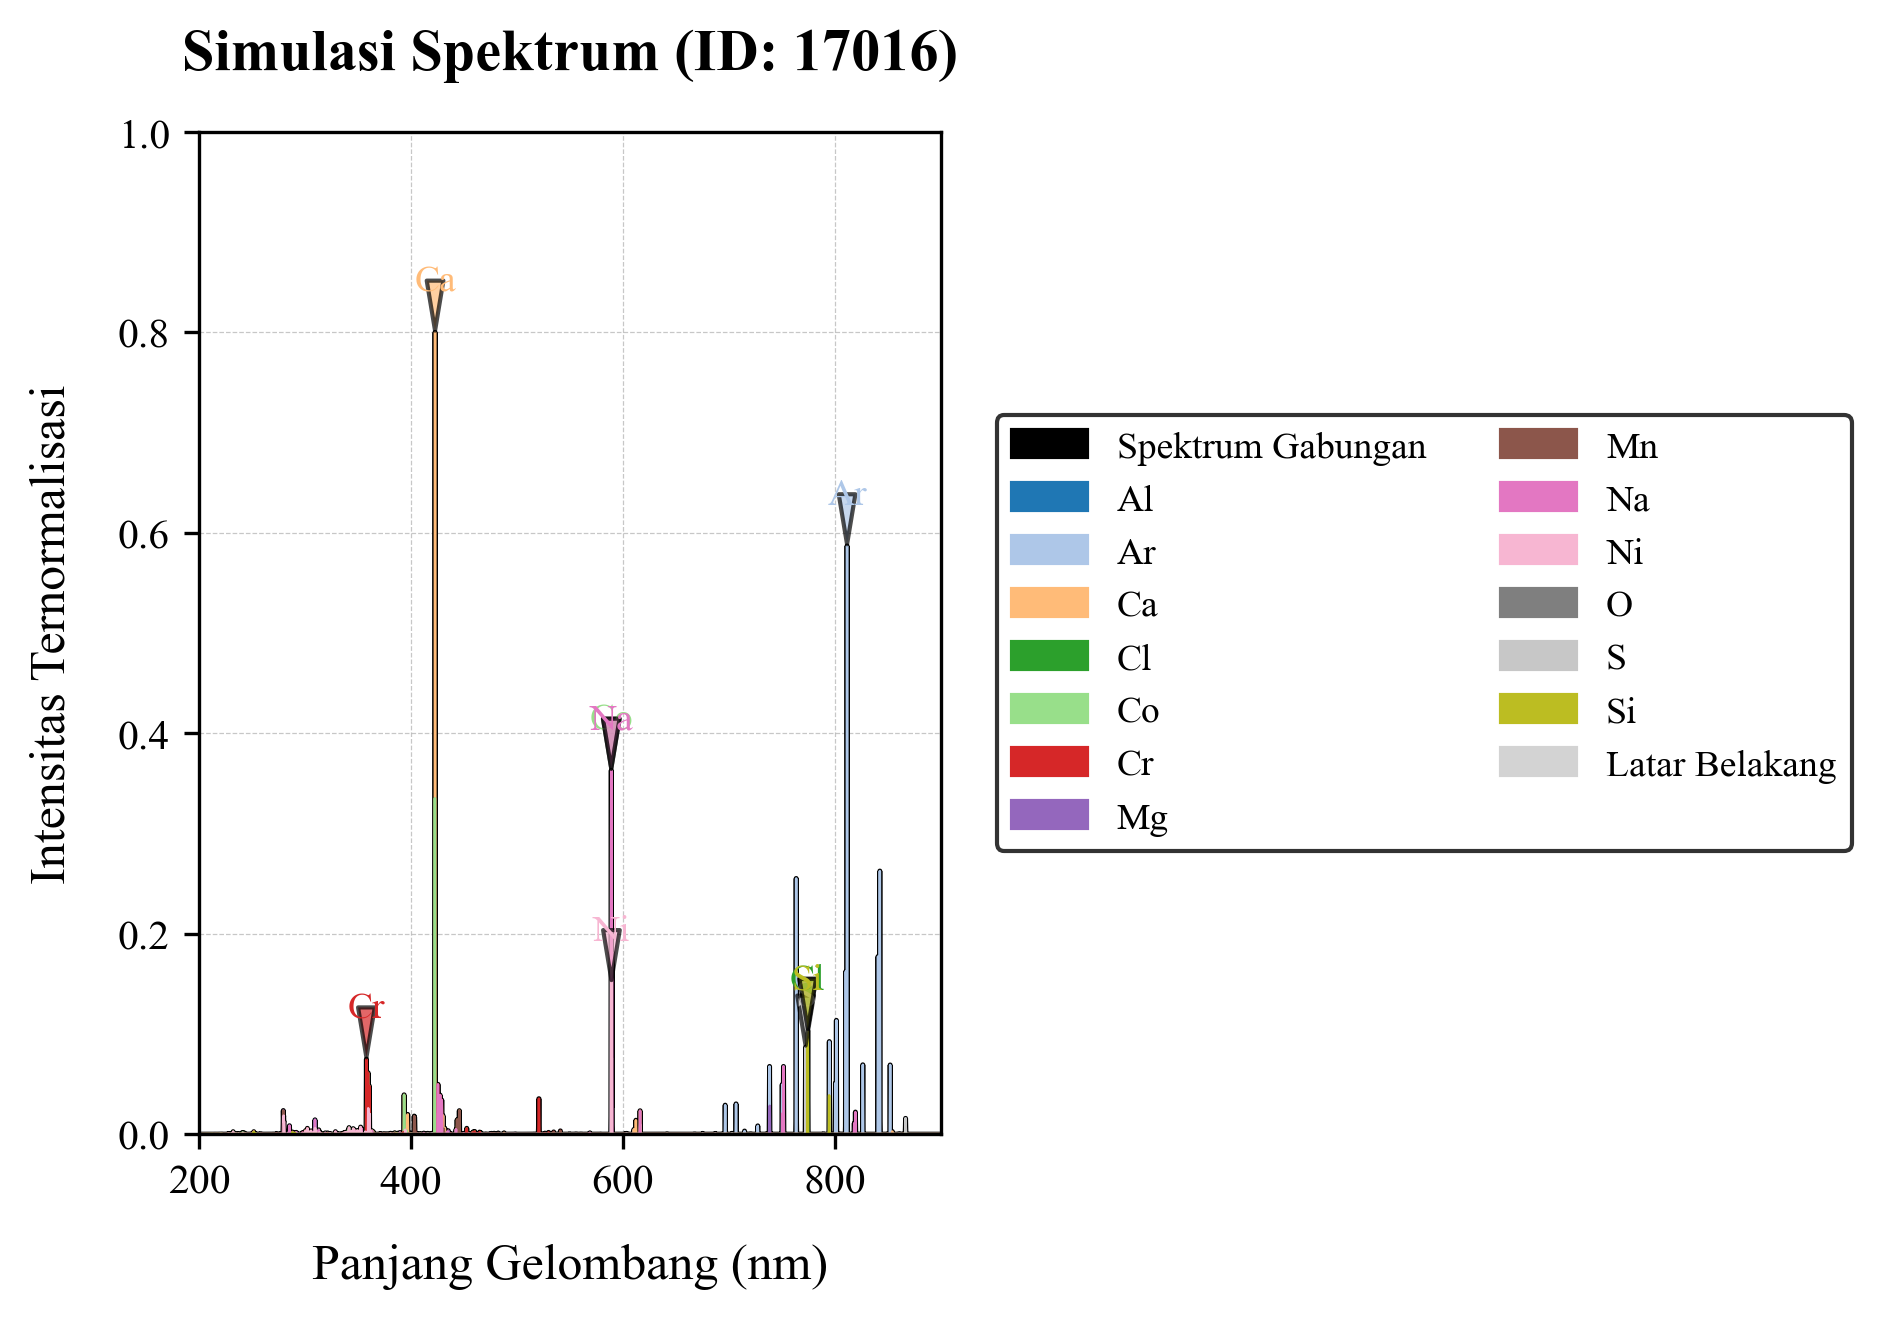
\includegraphics[width=\textwidth]{spectrum_17016.png}
        \caption{Spectral simulation plot for sample 17016 in full horizontal layout.}
        \label{fig:spectrum_17016}
    \end{landscape}
\end{figure}

\clearpage

\end{document}
